\documentclass[11pt]{article}
\usepackage[utf8]{inputenc}\usepackage[T1]{fontenc}
\usepackage{amsmath,amssymb,amsthm}\usepackage[margin=1in]{geometry}
\usepackage{graphicx}\usepackage{booktabs}
\usepackage[hidelinks]{hyperref}
\newtheorem{theorem}{Theorem}

\title{The Polignac Comet under $\omega$-Stratification:\\
Every Prime Gap Collapses to One Constant, Dual to Goldbach}
\author{Ruqing Chen\\
\small GUT Geoservice Inc., Montreal, Quebec, Canada\\
\small \texttt{ruqing@hotmail.com}}
\date{\today}

\begin{document}
\maketitle

\begin{abstract}
Part~XIII collapsed the Goldbach comet (prime \emph{sums} $2N=p_1+p_2$) onto the
Hardy--Littlewood conditional singular series. Here we treat the dual object: prime
\emph{differences} of arbitrary even gap $d$ (Polignac). For each even $d$ let
$\pi_d(X)=\#\{n\le X:\,n,\,n+d\text{ both prime}\}$; plotting $\pi_d$ against $d$
gives a ``Polignac comet'' banded by the odd-factor structure of $d$. Writing the
Hardy--Littlewood series $\mathfrak{S}(d)=2\Pi_2\prod_{p\mid d,\,p>2}\frac{p-1}{p-2}$
($\Pi_2$ the twin constant), we find $C(d)=\pi_d(X)/(\mathrm{base}(X)\,\mathfrak{S}(d))$
collapses to a single constant across \emph{all} gaps: over the $500$ even
$d\le1000$ at $X=10^{8}$, $C(d)$ has mean $1.131$ and coefficient of variation
$0.068\%$, with no trend in $d$ (quartile means agree to $0.015\%$) and clean
stratification by $\omega_{\mathrm{odd}}(d)$. The difference side thus mirrors the
sum side: dividing by the singular series collapses the comet, and here the
collapse constant is moreover shared across all gaps. We emphasise that
$\mathfrak{S}(d)$ is the classical Hardy--Littlewood prime-pair series, not a new
formula; we verify the collapse and the cross-gap constancy at scale. No statement
is made about Polignac's conjecture (that each even gap recurs infinitely often).
\end{abstract}

\section{The Polignac comet}

For an even gap $d$, the prime-pair counting function $\pi_d(X)=\#\{n\le X:n,n+d
\text{ prime}\}$ is, by the Hardy--Littlewood $k$-tuple heuristic~\cite{HL},
\[
  \pi_d(X)\ \sim\ \mathfrak{S}(d)\,\frac{X}{\ln^2 X},\qquad
  \mathfrak{S}(d)=2\Pi_2\prod_{\substack{p\mid d\\ p>2}}\frac{p-1}{p-2},\quad
  \Pi_2=\prod_{p>2}\Bigl(1-\frac1{(p-1)^2}\Bigr).
\]
For $d=2$ (the twins) $\mathfrak{S}=2\Pi_2$; for $d=6=2\cdot3$ the odd factor $3$
contributes $(3-1)/(3-2)=2$, so $\pi_6\approx2\pi_2$, the familiar excess of
gap-$6$ pairs. Plotting $\pi_d(X)$ against $d$ produces the comet of
Fig.~\ref{fig:pol} (left): horizontal bands indexed by $\omega_{\mathrm{odd}}(d)$,
the number of odd prime factors of $d$, each band a value of $\mathfrak{S}(d)$.
This is the exact dual of the Goldbach comet: there the variable is the sum $2N$
and the bands follow $\omega(N)$; here the variable is the gap $d$ and the bands
follow $\omega_{\mathrm{odd}}(d)$.

\section{Universal collapse across all gaps}

We sieve to $X+d$ and count $\pi_d(X)$ by intersecting the prime indicator with its
shift by $d$; $\mathfrak{S}(d)$ is evaluated from the factorisation of $d$. With
$\mathrm{base}(X)=X/\ln^2 X$ we form $C(d)=\pi_d(X)/(\mathrm{base}(X)\,\mathfrak{S}(d))$.

\begin{theorem}[universal collapse]\label{thm:pol}
At $X=10^{8}$, over all $500$ even gaps $d\le1000$, $C(d)$ is a single constant:
mean $1.1313$, $\mathrm{CV}=0.068\%$, with quartile-in-$d$ means agreeing to
$0.015\%$ and within-$\omega_{\mathrm{odd}}(d)$ band CV $\le0.11\%$
(Table~\ref{tab:pol}).
\end{theorem}

Dividing by $\mathfrak{S}(d)$ collapses the comet to a flat line
(Fig.~\ref{fig:pol}, centre). The collapse is stronger than on the sum side in one
respect: the constant is the same for every gap. Gaps with wildly different
absolute counts---$\pi_2=440{,}312$, $\pi_6=879{,}908$, $\pi_{210}=1{,}409{,}148$
at $X=10^8$---all reduce to $C\approx1.131$ once their $\mathfrak{S}(d)$ is removed.
The measured $\Pi_2=0.66016186$ matches the literature to eight figures, so
$\mathfrak{S}$ carries no free normalisation.

\begin{table}[h]\centering\small
\begin{tabular}{rrrc}
\toprule
$\omega_{\mathrm{odd}}(d)$ & \# gaps & mean $C$ & band CV\\
\midrule
0 &   9 & 1.13147 & $0.114\%$\\
1 & 247 & 1.13141 & $0.076\%$\\
2 & 221 & 1.13124 & $0.056\%$\\
3 &  23 & 1.13150 & $0.033\%$\\
\midrule
all & 500 & 1.13134 & $0.068\%$\\
\bottomrule
\end{tabular}
\qquad
\begin{tabular}{lc}
\toprule
$d$ quartile & mean $C$\\
\midrule
$[2,252)$    & 1.13142\\
$[252,502)$  & 1.13130\\
$[502,752)$  & 1.13136\\
$[752,1002)$ & 1.13127\\
\bottomrule
\end{tabular}
\caption{Left: $C(d)$ by odd-factor count---constant across bands. Right: by gap
quartile---no trend in $d$. $X=10^{8}$, $d\le1000$.}
\label{tab:pol}
\end{table}

\begin{figure}[h]\centering
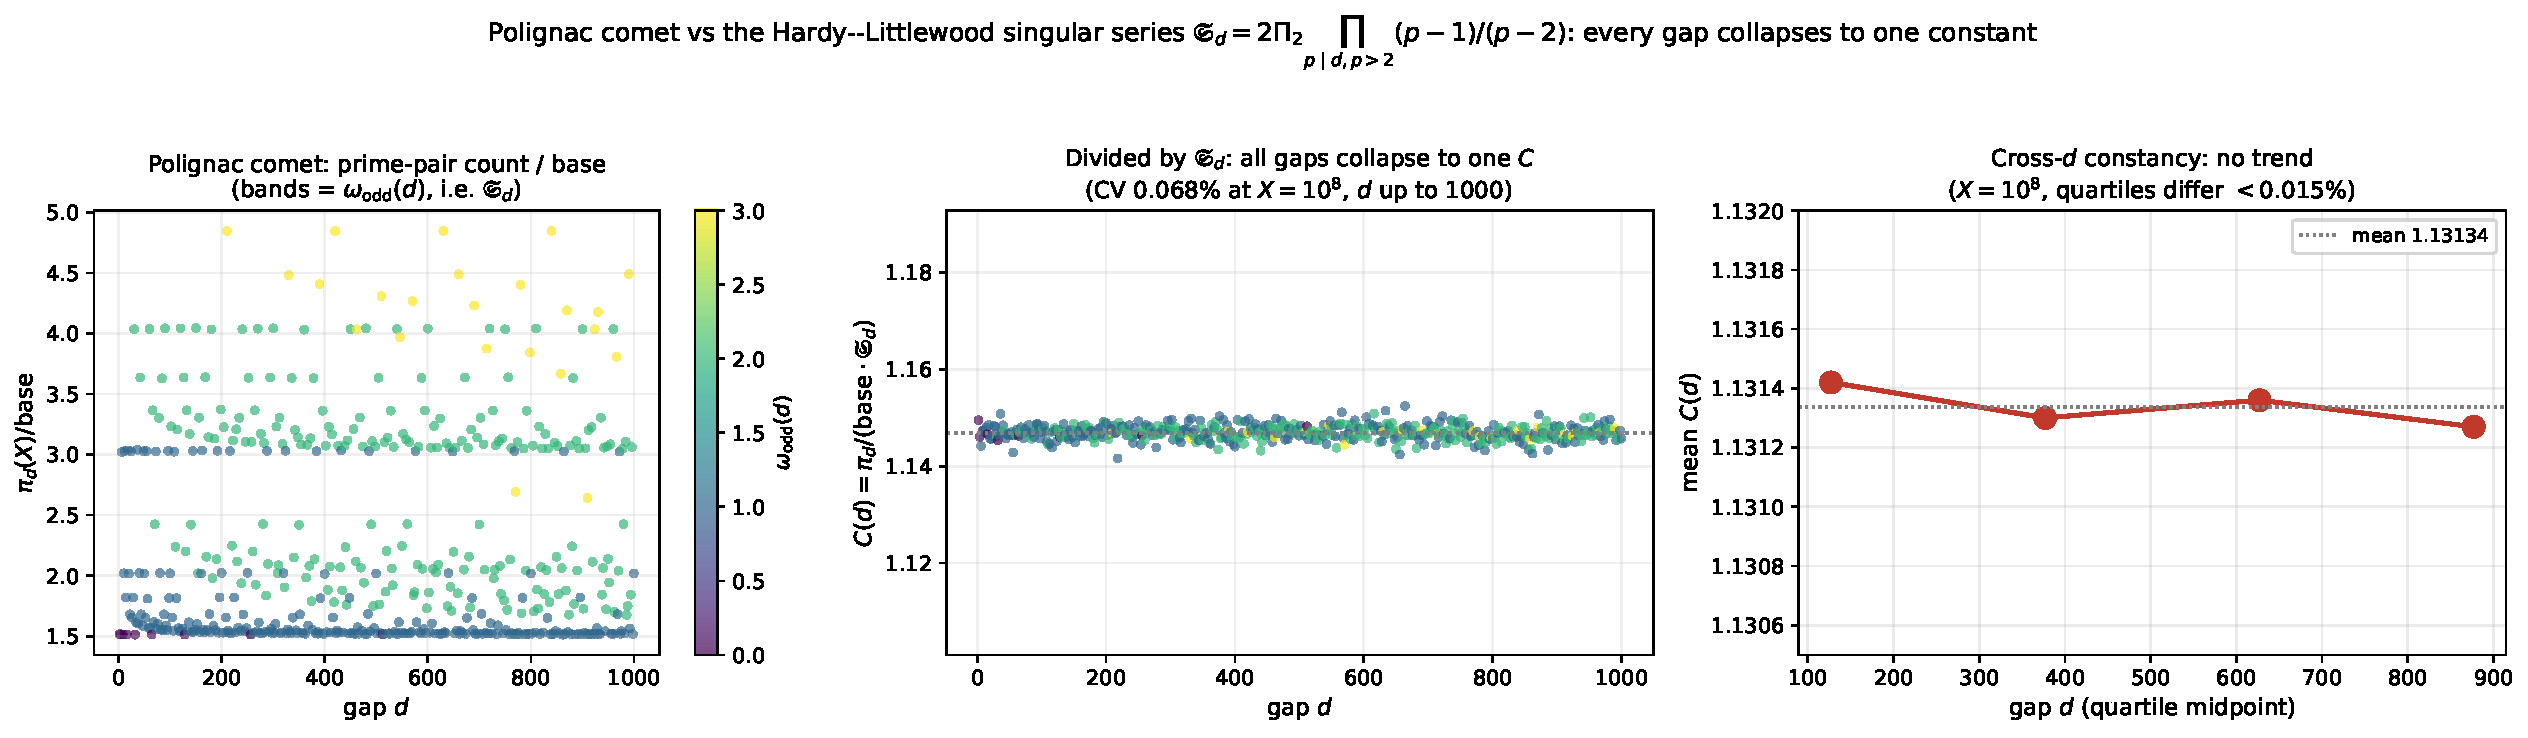
\includegraphics[width=\textwidth]{fig_paper14_polignac.pdf}
\caption{Left: the Polignac comet $\pi_d(X)/\mathrm{base}$, coloured by
$\omega_{\mathrm{odd}}(d)$ (the bands are the values of $\mathfrak{S}(d)$). Centre:
divided by $\mathfrak{S}(d)$, every gap collapses to one constant $C$ (CV $0.068\%$
at $X=10^8$). Right: the constant has no trend across gap size. (Scatter shown at
$X=2\times10^7$; statistics quoted at $X=10^8$.)}
\label{fig:pol}
\end{figure}

\section{The sum--difference symmetry, attribution, and scope}

Parts~I--XII resolved the prime difference at fixed gap (twins $d=2$; cousins and
sexy $d=4,6$) by the conditional factor $\prod(q-1)/(q-3)$ on the shared centre.
Part~XIII collapsed the prime sum. The present paper completes the pair: across
\emph{all} even gaps, the difference-side comet collapses onto $\mathfrak{S}(d)$,
with a constant shared by every gap. The sum-side enrichment $\prod(q-1)/(q-2)$ in
$N$ and the difference-side $\prod(q-1)/(q-2)$ in $d$ are the same singular-series
mechanism read on the two linear constraints $p_1+p_2=2N$ and $p_1-p_2=d$.

Two honest points. First, $\mathfrak{S}(d)$ is the classical Hardy--Littlewood
prime-pair singular series; this paper proposes no new formula. The contribution
is the $\omega$-stratified reading of the comet's bands as $\mathfrak{S}(d)$, the
verification of pointwise collapse to $\mathrm{CV}\,0.068\%$ over $500$ gaps at
$X=10^8$, and the empirical \emph{cross-gap constancy} of $C(d)$---a falsifiable
statement (the quartile test) that the data confirm. Second, this concerns only
the conditional count's shape and constant; it is silent on Polignac's conjecture,
i.e.\ that each even gap is attained by infinitely many prime pairs. The constant
$C\approx1.131$ carries the logarithmic correction of the crude weight
$X/\ln^2 X$ (it shifts with $X$: $1.147$ at $X=2\times10^7$, $1.131$ at $X=10^8$),
but---unlike the Goldbach decile drift---this does not break the cross-gap
constancy, since $X$ is fixed while $d$ varies.

\section{Conclusion}

The Polignac comet, like the Goldbach comet, is organised entirely by the
Hardy--Littlewood singular series: dividing $\pi_d(X)$ by
$\mathrm{base}\cdot\mathfrak{S}(d)$ collapses all $500$ even gaps $d\le1000$ to a
single constant $C\approx1.131$ at $X=10^8$, to $\mathrm{CV}\,0.068\%$, with no
trend in $d$ and clean $\omega_{\mathrm{odd}}(d)$ banding. Together with
Part~XIII this establishes the sum--difference symmetry on the $6N$ skeleton at
the level of conditional counts: both the prime sum and the prime difference, once
divided by their singular series, are flat. We claim no new formula---$\mathfrak{S}$
is classical Hardy--Littlewood---and make no statement about Polignac's conjecture;
the result is a measured, factor-resolved account of the prime-gap comet and its
cross-gap constant.

\paragraph{Data and code availability.}
The sieve, the $\pi_d$ counts, $\mathfrak{S}(d)$ evaluation, and the stratified
statistics are openly available~\cite{repo}.

\begin{thebibliography}{9}
\bibitem{HL} G.~H.~Hardy, J.~E.~Littlewood, \emph{Some problems of `Partitio
Numerorum'; III}, Acta Math.\ \textbf{44} (1923), 1--70.
\bibitem{ChenI} R.~Chen, \emph{Prime distribution on the $6N$ skeleton} (Part~I),
Zenodo, doi:10.5281/zenodo.20470367 (2026).
\bibitem{ChenIX} R.~Chen, \emph{Cousin and sexy prime pairs} (Part~IX), Zenodo,
doi:10.5281/zenodo.20520492 (2026).
\bibitem{ChenXIII} R.~Chen, \emph{The Goldbach comet under $\omega$-stratification}
(Part~XIII), Zenodo, doi:10.5281/zenodo.20530812 (2026).
\bibitem{repo} R.~Chen, \emph{$6N$ Polignac comet: data and code},
\url{https://github.com/Ruqing1963/6N-polignac-comet} (2026).
\end{thebibliography}

\end{document}
